%
% password manager? password management system?
%
% \documentclass{article}
\documentclass{sigchi}

\usepackage{balance}  % to better equalize the last page
\usepackage{graphics} % for EPS, load graphicx instead
\usepackage{times}    % comment if you want LaTeX's default font
\usepackage{url}      % llt: nicely formatted URLs

% \usepackage{times}
% \usepackage{uist}
% \usepackage{graphicx}

\usepackage{here} % [H]とするとその場所に配置されるらしい

% llt: Define a global style for URLs, rather that the default one
\makeatletter
\def\url@leostyle{%
  \@ifundefined{selectfont}{\def\UrlFont{\sf}}{\def\UrlFont{\small\bf\ttfamily}}}
\makeatother
\urlstyle{leo}


% To make various LaTeX processors do the right thing with page size.
\def\pprw{8.5in}
\def\pprh{11in}
\special{papersize=\pprw,\pprh}
\setlength{\paperwidth}{\pprw}
\setlength{\paperheight}{\pprh}
\setlength{\pdfpagewidth}{\pprw}
\setlength{\pdfpageheight}{\pprh}

% Make sure hyperref comes last of your loaded packages, 
% to give it a fighting chance of not being over-written, 
% since its job is to redefine many LaTeX commands.
\usepackage[pdftex]{hyperref}
\hypersetup{
pdftitle={SIGCHI Conference Proceedings Format},
pdfauthor={LaTeX},
pdfkeywords={SIGCHI, proceedings, archival format},
bookmarksnumbered,
pdfstartview={FitH},
colorlinks,
citecolor=black,
filecolor=black,
linkcolor=black,
urlcolor=black,
breaklinks=true,
}

% create a shortcut to typeset table headings
\newcommand\tabhead[1]{\small\textbf{#1}}

\begin{document}

\long\def\EP{\textsf{EpisoPass}}
\long\def\PW{password}
\long\def\SS{seed string}
\long\def\EM{episodic memory}
\long\def\SQ{secret question}

% Copyright notice ---
\conferenceinfo{UIST'16}{Tokyo}
\CopyrightYear{2016}
\crdata{x-xxxxx-xxx-x/xx/xxxx}

\title{EpisoPass: Password Management based on \\ Episodic Memories}

\numberofauthors{3}
\author{
  \alignauthor 1st Author Name\\
    \affaddr{Affiliation}\\
    \affaddr{Address}\\
    \email{e-mail address}\\
    \affaddr{Optional phone number}
  \alignauthor 2nd Author Name\\
    \affaddr{Affiliation}\\
    \affaddr{Address}\\
    \email{e-mail address}\\
    \affaddr{Optional phone number}    
  \alignauthor 3rd Author Name\\
    \affaddr{Affiliation}\\
    \affaddr{Address}\\
    \email{e-mail address}\\
    \affaddr{Optional phone number}
}

\maketitle

\begin{abstract}
% 忘れることがない{\EM}にもとづく{\SQ}を使って強力な{\PW}を生成/管理するシステム「\textsf{\EP}」を提案する。
% {\EP}は、ユーザが作成した{\SQ}への回答にもとづいて{\SS}を換字することによって{\PW}を生成する。
% {\SS}や回答のバリエーションにより異なる{\PW}が生成されるので様々なサービスに対して異なる{\PW}を生成できることに加え、
% {\SS}を逆計算することにより既存の{\PW}の管理もできる。
% 適切な運用により、{\PW}に関連するあらゆる情報を秘密にすることなく
% 強力な{\PW}の生成/管理が可能である。

%
% We introduce a password generation/management system called EpisoPass,
% which converts a seed string into a password using the user's
% episodic memories represented as a set of questions and answers
% which can be solved only by the user.
%
% Using EpisoPass with well-defined questions and answers,
% a user can always retrieve various passwords without worrying about
% remembering secret information.

We propose a password manager \textit{EpisoPass} that supports
generating strong passwords based on the user's secret and unforgettable
episodic memories.
%
To use EpisoPass,
a user first collects question-answer pairs related to his episodic memory
and registers them with fake answers.
%
When the user wants to generate a password,
EpisoPass shows the questions and lists of possible answers and asks
the user to select correct ones.
Then EpisoPass generates a password by substituting characters of the
seed string based on the selected answers.
%
If the user is the only person who knows the correct answer,
% If the right answers to the questions are known only to the user,
the password cannot be guessable by other people, and
various strong passwords can be easily managed
without using master passwords or secret devices that are
usually required on conventional password managers.
%
\end{abstract}

\keywords{
  Passwords; password managers; episodic memories; EpisoPass;
%	keywords should be separated by a semi-colon. \newline
%	\textcolor{red}{Optional section to be included in your final version, 
%  but strongly encouraged.}
}

\category{H.5.2.}{Information Interfaces and Presentation (e.g. HCI)}{User Interfaces}
\category{K.6.5.}{Management of Computing and Information Systems}{Security and Protection}

\tolerance=400 
  % makes some lines with lots of white space, but 	
  % tends to prevent words from sticking out in the margin

\section{INTRODUCTION}

% Passwordは使われている
% 
% Passwordが辛いのは一般的事実である[?]
%   基本的に強くするには長くしなければならない
%   忘れる
%   覚えられない
%   サービスごとにパスワードは変えるべきである[?] でも無理
%   定期的に更新させられる
% 強いパスワードを頭で覚えて管理するのは不可能
%       特に弱者には
%   パスワード作成アルゴリズムを自力で使っている人もいるがそれは難しい

Passwords have been used for various Web services and applications
for a long time, and currently the most popular authentication method on the Internet.
%
Since short passwords are easily guessed by attackers and
using the same password for different services is unsafe,
different long passwords should be used for different services.
However,
remembering many long passwords is almost impossible for ordinary humans.
%
% According to Flor\^{e}ncio,
According to a research in 2007,
people use 6.5 passwords on 25 Web services on average, and
4.28\% of the users forget their passwords in 3 months\cite{Florencio:2007:LSW:1242572.1242661}.

%また2011年の野村総研の調査によれば、
%一般的なユーザが{\PW}認証を行なうサイトは平均19.4個で、
%利用している{\PW}は平均3.1個であった\cite{野村総研}。
%多数の{\PW}を記憶することが困難であるため、
%多くのユーザが同じ{\PW}を複数サイトで使い回しているのだと思われる。

% People are frequently asked to register a password when
% they try to use a new service.

% もっと別の認証もいろいろ提案されている
%   画像認証[MALASYM][その他いろいろ]
%   
%   特殊ハードのような持ち物を使う方法など[Pico][YubiKey][RSA]
%   生体認証 指紋認証
%   行動からの認証[]
%   位置ベースの認証[SOUPS]
%  完全置き換えはしばらくは不可能だろう

Since passwords are difficult to handle,
various other authentication methods have been proposed.
For example,
image-based authentication\cite{Biddle:2012:GPL:2333112.2333114}\cite{GraphicalPasswords}, 
biometrics authentication\footnote{
  % \textsf{https:{\slash}{\slash}en.wikipedia.org{\slash}wiki{\slash}Biometrics}
  \url{https://en.wikipedia.org/wiki/Biometrics}
},
behavior-based authentication\cite{Dandapat:2015:AYD:2702123.2702457}, 
and many other authentication methods have been proposed.

% というのもパスワードには利点があるから[Bonneau]
%   すでに普及
%   KB以外の特殊ハードが要らない
%   アタック方法はいろいろあるし[] 流出もしばしばだが
%     うまく実装したシステム上でうまく使えば安全
%     ハッシュ、ソルト
%     実装が比較的簡単
% なのでパスワードが近い将来死滅するとは考えられない

However,
password-based authentication is still the most
convenient and strong method\cite{Bonnearu:ReplacePasswords},
and it is not supposed to get extinct
in a short period of time\cite{Herley:2009:PSS:1601990.1602010}.

% % なのでパスワードと生きる方法が工夫されている
% %   強いパスワードを考える方法[]
% %     覚える方法が提案されてたり[Bonneau]
% %       万人むけはむり

% パスワードが死滅しないならパスワードと生きる方法が必要である
%   たとえば様々なパスワード管理システム[][][][]の利用がすすめられている
%   しかしマスターパスワードがいったり特殊ハードがいったりする
%   特殊システムがいる場合がある
%   特殊ハードやソフトは利用がどうしても難しい

If we have to live with password-based authentication systems,
we have to devise some ways to handle many passwords, and
various ``password managers'' have been proposed
\cite{OnePassword}%
\cite{Dashlane}%
\cite{ミルパス}%
\cite{LastPass}%
\cite{KeyPass}%
\cite{NortonIDSafe}%
\cite{IDManager}.
%
Password managers remember users' passwords and help them enter
passwords on various services.
%
%{\PW}管理システムは
%ひとつの「マスター{\PW}」を利用して他のすべての{\PW}を管理するもので、
%暗号化されたデータベースに{\PW}を格納するもの%
%
Most password managers can manage various passwords by
asking users to remember a single ``master password'' to access the database.
%
%が多いが、サービス名をもとにマスター{\PW}を変換することによって
%複数の{\PW}を生成するシステム\cite{SuperGenPass}もある。
%両者ともにマスター{\PW}の記憶は必須であり、
%マスター{\PW}を盗まれたり忘れたりする危険がある。
%
Although password managers are useful,
users have to remember the master password
or use a special hardware device
for safely handle password managers, and
password managers usually run on limited devices.

% 読みとることができない脳内情報を利用するという基本手法は良いのだが覚えられないのが問題である
%   だとすると...パスワードを記憶するかわりに、****脳が既に覚えている秘密の記憶からパスワードを生成すればよいはずである***
%   確かな脳内情報を使ってパスワードを利用する必要があるが、
%     沢山の強力なパスワードそのものを覚えることは不可能に近い
%   だとすると、確かな脳内秘密情報からパスワードをGenerateするしかない
%   そこでエピソード記憶を使う
%   秘密の知識からGenerateするとよい
%

If we don't want to carry any special device for authentication,
all the information required for the authentication should be
kept in the brain.
%
However, the biggest problem of brain-based authentication is that
users cannot safely keep memories like long passwords or master password.
For this reason, we believe that
it is far better to ``generate'' something for the authentication,
based on users' episodic memories which they can never forget.
%
% We believe that a password manager should have the following features.
% (1) It should be available on any platform including PCs, smartphones, and the Web.
% (2) Users should not have secret information (e.g. master password) or special device.
% (3) Rely only on the information in the user's brain.
%
We propose a password manager \textit{EpisoPass} that generates strong passwords
based only on the user's secret episodic memories that the user can never forget.

\section{EpisoPass}

EpisoPass is a password manager that supports generating
strong passwords based on users' secret episodic memories.
%
% Before using EpisoPass for generating passwords,
% a user provides a seed string and many question-answer pairs to EpisoPass,
% and a password is generated based on the user's selections.
%
Memories in human brain are not uniform.
Some memories are very short-lived, and others are unforgettable.
When we have a very impressive experience,
that memory will stay in the brain for a long time and
cannot easily disappear.
On the other hand, when we study math and try to remember a formula,
it is usually hard to memorize it unless we practice a lot,
since the knowledge about the formula is not related to
any personal experiences.
The former type of memory is called the episodic memory and
people cannot easily lose it.
Memories of passwords belong to the latter type and
people cannot easily remember them, just like people cannot
remember math formulas easily.
%

% \begin{quote}
% Episodic memory is the memory of autobiographical events (times,
% places, associated emotions, and other contextual who, what, when,
% where, why knowledge) that can be explicitly stated. It is the
% collection of past personal experiences that occurred at a particular
% time and place. For example, if one remembers the party on his or her
% 6th birthday, this is an episodic memory. They allow an individual to
% figuratively travel back in time to remember the event that took place
% at that particular time and place.[1]
% 
% Semantic memory is one of the two types of declarative or explicit
% memory (our memory of facts or events that is explicitly stored and
% retrieved).[1] Semantic memory refers to general world knowledge that
% we have accumulated throughout our lives.[2] This general knowledge
% (facts, ideas, meaning and concepts) is intertwined in experience and
% dependent on culture. Semantic memory is distinct from episodic
% memory, which is our memory of experiences and specific events that
% occur during our lives, from which we can recreate at any given
% point.[3] For instance, semantic memory might contain information
% about what a cat is, whereas episodic memory might contain a specific
% memory of petting a particular cat. We can learn about new concepts by
% applying our knowledge learned from things in the past.[4] The
% counterpart to declarative, or explicit memory, is procedural memory,
% or implicit memory.[5]
% \end{quote}

Password generation on EpisoPass is performed through the following steps:

\begin{enumerate}
\item A user registers many question texts related to the user's personal
secret episodic memories that the user never forgets,
and provides a correct answer and additional fake answers.

\item The user provides a long ``seed string'' for each service that requires
a password.

\item EpisoPass shows the data to the user so that
the user can select the right answer for each question.
Based on the user's selections,
EpisoPass substitutes characters in the seed string and generates
random-looking password candidate strings.
After selecting all the right answers,
the user copies the calculated string
and register it as the password for the service.
\end{enumerate}

\subsection{Using EpisoPass on a browser}

Figure \ref{web1} shows how to generate a password
on EpisoPass running on a browser.
Many questions related to the user's episodic memories are shown to the user,
and many candidate answers are also shown for each question.
When a user clicks and selects one of the answers for each question,
the seed string shown at the top-left is converted to a random-looking string
based on the selections.
When the user selects the right answers to all the questions,
the right password is calculated and shown at the top.

% If the q-a is based on the user's episodic memories and
% nobody knows the correct answer,
% only the user can select the set of right answers and
% use the converted string as the password.

\begin{figure}[t]
\centering
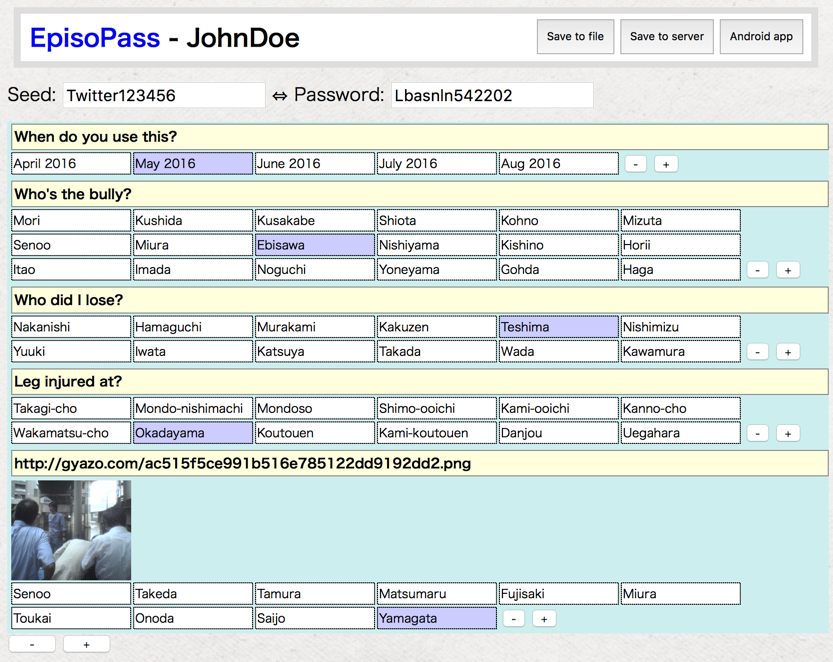
\includegraphics[width=1.0\columnwidth]{figures/c1bd6e7f67698c70978f528ccd2339d9}
\caption{Generating a Twitter password with EpisoPass.}
\label{web1}
\end{figure}

In Figure \ref{web1},
``\textsf{Twitter123456}'' is provided as the seed string,
and according to the selections to the five questions,
the seed string is converted to a string
``\textsf{Lbasnln542202}'',
which can be used as the password for Twitter.

When the user clicks another candidate,
the seed string is converted to another strings like
``\textsf{Bhtuyna904127}'' (Figure \ref{web11}).

\begin{figure}[H]
\centering
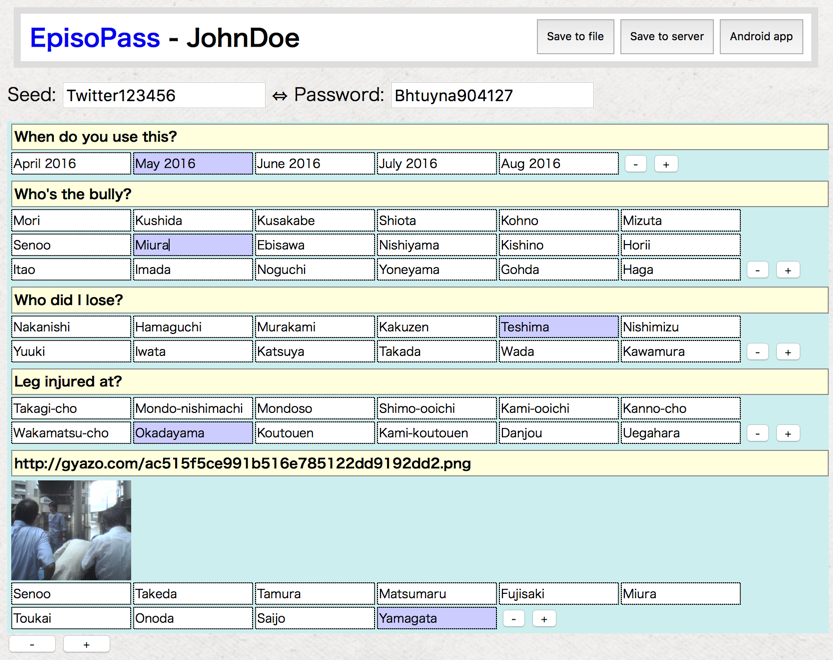
\includegraphics[width=1.0\columnwidth]{figures/01e5507d090eb494a20bcbc47c86b1d2}
\caption{Selecting a different answer.}
\label{web11}
\end{figure}

In this way, different selections yields different password strings and
the password string generated after selecting correct answers can be
used as the password for the service.

Capital letters in the seed string are substituted to capital letters in the password,
and digits in the seed string are substituted to digits,
so that generated passwords conforms to password character restrictions
sometimes requested by the service.

% {\SS}として「\textsf{Twitter123456}」という文字列を指定しており、
% 4個の{\SQ}に対する回答選択に応じて
% 「\textsf{Mfveabn574923}」のような{\PW}候補が生成される。
% 異なる答をを選択すると全く異なる文字列が生成される。
% {\SS}の8文字目が数字である場合は{\PW}の8文字目も数字になるなど、
% {\SS}の文字種に対応した{\PW}候補が生成される。

The second question in Figure \ref{web1}
is based on the author's episodic memory at elementary school,
and the last question is related to a more recent event
which the author thinks he can never forget.
All the questions are related to the author's episodic memories
that he thinks he never forgets, and nobody else knows which one of the
candidate answers is the right one.

Questions and answers can be edited directly on the browser, and they can be
saved on the server by clicking the ``save to server'' button.
The Q-A data sets are saved on the server,
but no information about the correct answer or the
generated password is saved on the server.

% {\SQ}と答はブラウザで編集でき、
% 右上の「サーバにセーブ」ボタンを押すことにより{\SS}、秘密の問題、答のリストがサーバにセーブされる。
% 「ファイルにセーブ」ボタンを押すとJSONデータをパソコンにダウンロードでき、
% パソコン上のJSONデータをブラウザにドラッグ\&ドロップするとサーバにアップロードできる。
% ユーザはどれが正答かを指定するわけではないので
% 問題データを見てもユーザの{\PW}はわからない。

When we change the secret string to ``\textsf{Facebook123456}'',
the generated password changes to ``\textsf{Zxghfbqu533131}'',
as shown in Figure \ref{web2}.
In this way, we can generate different passwords for
different services just by changing the seed string.

\begin{figure}[H]
\centering
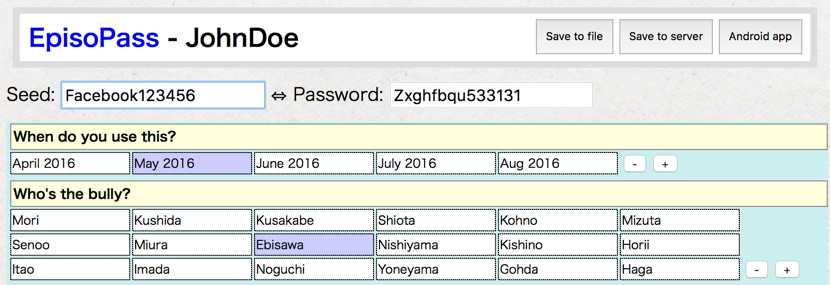
\includegraphics[width=1.0\columnwidth]{figures/0e2820c279afc70520482e0fc53b6ed9}
\caption{Generating the password for FaceBook.}
\label{web2}
\end{figure}

% {\PW}文字列の計算方法}
% 問題と回答から文字列を生成し、そのMD5値によって{\SS}を換字することにより
% {\PW}を生成している。
% {\PW}文字列の計算方法は附録に示す。

%アルゴリズムはここ? Algorithm

Character substitution is performed based on the hash value
calculated from concatinating all the selected answers.
For example, if the user selects ``\textbf{\texttt{Ebisawa}}'' to the question ``\textbf{\texttt{Who's the bully?}}'',
a hash value calculated from  ``\textbf{\texttt{Who's the bully:Ebisawa}}''
is used for the substitution.
Details of the algorithm is shown in the Appendix.

% 問題と回答から文字列を生成し、そのMD5値によって{\SS}を換字することにより
% {\PW}を生成している。
% {\PW}文字列の計算方法は附録に示す。

% \subsubsection{回答選択により{\PW}を切り換え}
% \label{pwgen}
% 
% サービスごとに{\SS}を変えるのではなく、
% 図\ref{web3}のように
% サービス名に応じて回答を変えることによって異なる{\PW}を作成することも可能である。
% {\PW}としての長さや文字種に特種な制約が無いサービスに関してはこの方法が便利である。
% 
% \begin{figure}[H]
% \centerline{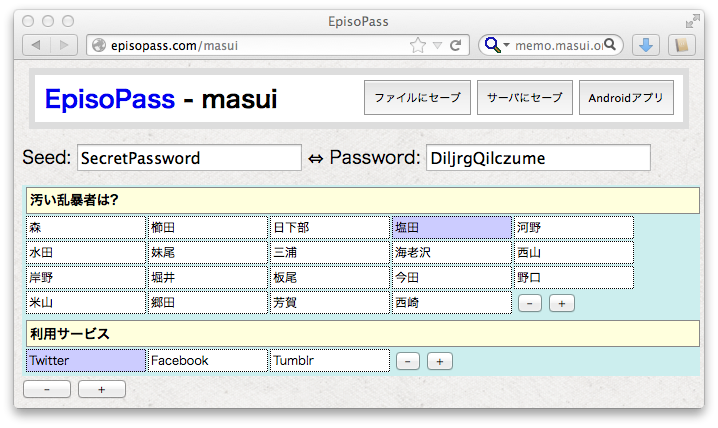
\includegraphics[width=83mm,bb=0 0 718 428]{../WISS/figures/a9167a6ec6af9c70dd1617e3fc25ec30.png}}
% \centerline{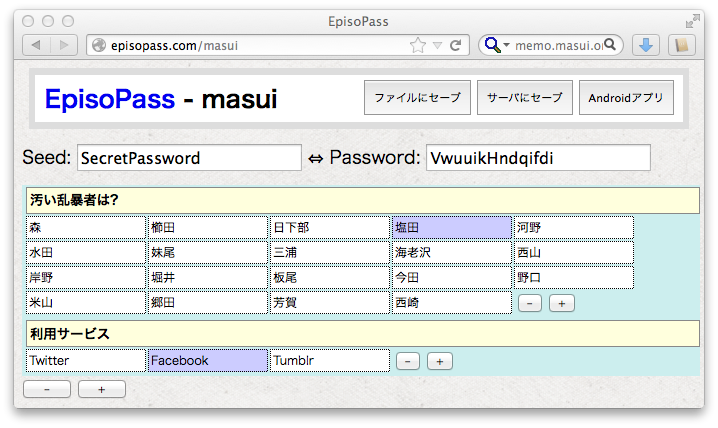
\includegraphics[width=83mm,bb=0 0 718 428]{../WISS/figures/5b887fabeb8e3319623901fe4a6c56f2.png}}
% \caption{サービス名に対応する回答で異なる{\PW}を生成.}
% \label{web3}
% \end{figure}

% 定期的に{\PW}変更を求められるシステムでは、
% 「利用期間は?」という質問に対して
% 「2013/1」「2013/2」のような答を用意しておけば、
% 時期を選択することによって簡単に{\PW}を変更することができるので便利である。

\subsection{Android application}


% Webサービスを利用する場合、ブラウザとサーバとの間の通信を
% 記録されたり盗み見されたりされる心配を完全に払拭することはできない。
% % 危険を完全になくすことはできない。
% 前述の例において、
% {\PW}はブラウザ内部でJavaScriptにより生成されるので、
% 一度ページを表示した後は
% ネットワークを遮断しても{\PW}計算を行なえるようになっているが、
% 最初から全く通信を行なわずに{\PW}を作成できる方がより安心であろう。
% このため、通信を全く行なわずにマシン単体で{\PW}計算を行なうための
% Androidアプリを用意した。
% ページの右上の「Androidアプリ」ボタンを押すと、
% 現在表示している秘密の問題と答を内蔵したAndroidアプリが
% サーバ上でビルドされてダウンロードされる。

If a user doesn't like to use EpisoPass service on the Net,
he can use an EpisoPass application on Android
which does not require network connection.
After registering questions and answers on the EpisoPass service,
the user can download an Android application from the server
by clicking the ``Android app'' button.
The application contains all the information required for generating passwords.
(The application is compiled and built on the server.)

% Android端末でアプリを実行すると図\ref{android1}のような画面が表示される。
% {\SS}を設定して「開始」ボタンを押すと図\ref{android2}のように質問がひとつずつ表示され、
% ボタンを押してすべて回答すると{\PW}が計算され図\ref{android3}のように表示される。

When the user runs the application and selects the right answer
to each question, he can eventually get the password and copy it to the password entry.
(Figure \ref{android1},\ref{android2})

\begin{figure}[H]
\centering
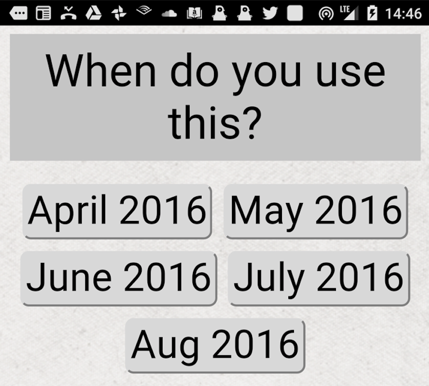
\includegraphics[width=0.7\columnwidth]{figures/429eec261024dc6c85351f51c12f09b4}
\caption{Running EpisoPass on Android.}
\label{android1}
\end{figure}

\begin{figure}[H]
\centering
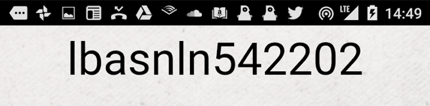
\includegraphics[width=0.7\columnwidth]{figures/ba8f5aeaa935ad63437969f4d746746b}
\caption{After finishing selections.}
\label{android2}
\end{figure}

% 回答入力と{\PW}計算はAndroid端末で実行されるため、
% 端末を「機内モード」に設定するなどの方法で
% ネットワーク接続を遮断した状態でも{\PW}を計算することができる。
% {\EP}をインストールしたAndroid端末を持っていれば常に各種の{\PW}を計算できるので、
% 他人のマシンや公共の場所に設置されたパソコンなどでも
% 容易にtwitterなどのネットサービスを利用することができる。

% The calculation is performed on Android without network connection,
% and the user can safely generate passwords 
% without feeling the fear of ...

% 前述の方法で{\EP}アプリをサーバからダウンロードする場合は、
% ブラウザ上で秘密の問題をサーバに登録する必要があるが、
% 秘密の問題を全くネット上に露出することなくアプリを利用することもできる。

\section{DISCUSSIONS}

In this section, we discuss the advantages and caveats of
using EpisoPass.

\subsection{Unforgettability}

The biggest advantage of using EpisoPass is that
users don't have to remember passwords of any kind and
they can stop worrying about password-related troubles.
%
Users of EpisoPass can save the seed string and question-answer data
at any place, and easily generate passwords by running
EpisoPass and answering questions.
If the question is based on old unforgettable episodic memories,
there is little chance of losing passwords.
If the user's memory is related to an episode of 20 years ago and the user clearly
remembers the episode now, it is unlikely that he forgets the episode 10 years later.

\subsection{Security strength of EpisoPass}

The strength of the generated password depends on the number of
questions and the secret level of the questions.
%
There have been many studies on the strength of passwords
\cite{Hayashi:2011:DSP:1978942.1979326}%
\cite{Komanduri:2011:PPM:1978942.1979321}, % どういうパスワードが強いか
but the strength of secret questions has not been studied enough.
%
% {\EP}で選択枝が10個の{\SQ}を8個使用する場合、
% 総当たりで{\PW}を生成するには
% 1億($10^8$)通りの試行が必要であり、
% % エントロピーは26.6 ($ = 8 \times \log_2 10$) ビット
% エントロピーは26.6ビットとなる。
%
When we use 10 secret questions with 20 answers and
there's no clue for the answer,
1 billion ($20^10$) trials should be performed to check
all the combinations of the answers,
and the entropy of the system is 43.2 ($10 \times \log_2 20$) bits.  % 10.0 * (Math.log(20.0)/Math.log(2.0))
%
% 英字からランダムに8文字を並べて作成した{\PW}のエントロピーは37.6ビットになるが、
% ``\textsf{pmvixuzq}''のように全く意味のない{\PW}を記憶して利用することは少ないため、
% 実際に利用される{\PW}のエントロピーは20ビット程度と考えられているので\cite{NIST}、
% {\SQ}と選択枝の数を10個程度用意すれば
% 通常の{\PW}と同程度の強度が期待できることになる。
%
It is almost the same entropy as using random 8-character English alphabets
as a password, in which case the entropy is 45.6 bits.
This level is considered to be strong enough for Web services,
where online brute-force attack is impossible\cite{Florencio:2007:SWP:1361419.1361429}.

\subsection{Selecting good questions}

% {\EP}利用において{\SQ}の選択は非常に重要である。
% 他人が推測することが難しく、自分が決して忘れないような{\EM}を{\SQ}として利用すべきであり、
% 以下のような性質をもつ記憶は{\SQ}として利用すべきではない。

The quality of the questions is the key to using EpisoPass.
If the episode is shared by someone else,
that person can easily answer the question and generate the
password just like the user.
%
The episode related to each question should not be known to other people,
and the episode should be unforgettable.
%
Finding such episodes seems difficult at first, but
when we try to remember experiences of old days,
we can recall many trivial episodes which are unforgettable but
not important to other people.
%
Old experiences like the following are candidates for
good questions used in EpisoPass.

\begin{itemize}
\item Memory of small injury. (Nobody cares it but you.)

\item Memories of bad experience like blunders or defeat.
(You don't tell it to anybody.)

\item Experience of finding a small special item which only you are interested in.
\end{itemize}

For example, a question like
``who hit you when you were 6 years old?''
is about a trivial experience that people do not mention,
but a bad experience like this is not forgettable.

Questions like ``Which food do you like best?'' should be avoided,
since some of the friends might know the user's taste.
Questions related to an episode which the user is proud of should also be
avoided, since the user might talk about the episode to somebody else.

We usually don't tell our bad trivial experiences to other people,
but we might boast of good experiences or even write a blog about it.
Also, our tastes (e.g. favorite food) might change in the long run.
Using such episodes for questions should be avoided.

% \begin{itemize}
% \item \textsf{自慢になるもの
% (何かの機会にうっかり他人に話してしまう可能性がある)}
% 
% \vspace{-1mm}
% \item \textsf{ネット上に記録が残っているもの}
% 
% \vspace{-1mm}
% \item \textsf{他人と情報を共有しているもの}
% 
% \vspace{-1mm}
% \item \textsf{趣味や嗜好に関連するもの
% (他人に推測されやすいうえに嗜好が変化する可能性がある)}
% 
% \end{itemize}

\subsection{Creating fake answers}

% {\SQ}の種類によっては偽答の生成が難しい場合がある。
% 図\ref{atmega}は電子工作に関する{\SQ}の例であるが、
% 正答と区別がつかない偽答を充分リストすることは難しい。

It is difficult to provide enough number of fake answers to a question like
``what was your favorite sport?''
because possible answers are limited.
%
% \begin{figure}[H]
% \centerline{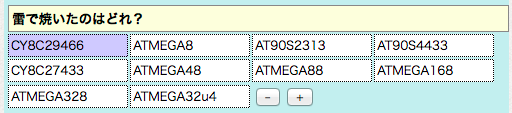
\includegraphics[width=83mm,bb=0 0 512 113]{../figures/2f63ceb9ab6faf8d81393953f2f95a8c.png}}
% \caption{偽答の生成が難しい例.}
% \label{atmega}
% \end{figure}
%
% 一方、正答として人名や地名を利用する場合、
% 正答に似た人名や地名をリストすることは難しくない。
% 「世田谷」が正答であるとき、
% 「目黒」「杉並」のような偽答を用意するのは簡単である。
%
On the other hand, if the right answer to the question is a name of a place or a person,
generating similar answers is easy.
For example, if the answer to the question is ``Colorado'',
we can easily provide fake answers like ``California'', ``Utah'', etc.
because we can use the list of states in the U.S.

% 正答と同じカテゴリに属する単語を自動的にリストすることができれば
% 正答をもとにして簡単に偽答のリストを生成することができる。
In this way, fake answers can be easily generated
if it is possible to collect words which belong to the same
category as the right answer.
%
% ひとつの単語もしくは単語の集合と同じカテゴリに属する単語を検索する手法は
% 「同位語検索」と呼ばれ、
% Webのデータを利用した様々な同位語検索システムが提案されている%
Various methods have been proposed for collecting words in the
same category, mainly for information retrieval tasks%
\cite{Huang:2012:LFC:2426725.2426728}% 読んでないけど
\cite{BooWa}% Boo!Wa!というサイトをやっている
\cite{Wang:2007:LSE:1441428.1442086}.% BooWa
%\cite{大島裕明:2006-12-15}.% ライバルサーチ「やーやら」
We can use such techniques for getting similar names.

\subsection{Universality}

Although everyone has to use authentication systems on the Internet these days,
not all the people are good at handling passwords.
Even experienced computer users have trouble with passwords,
since choosing a good password is not intuitive and
people forget passwords frequently.
%
Using EpisoPass, people can use password-based systems without knowing
techniques for creating and remembering strong passwords.
They only have to provide
questions and answers based on secret episodic memories.
%
By integrating EpisoPass into existing password-based services,
people can even use services without noticing that passwords are
required for the service.

\subsection{Frequent password update}

On many services, users are requested to change passwords periodically
to strengthen security.
%
% A user can generate a new strong password by using a randam character generator
% on a password manager, but he might want to old passwords in case some trouble happens.
%
Using EpisoPass, users can just provide a date-related question
like the first question shown in Figure \ref{web1},
and generate different strong passwords based on the answer.
Using this technique, people can easily manage old and new passwords.

\subsection{Comparison with challenge-response authentication}

% 一方、{\SQ}を利用する認証の脆弱性を利用した攻撃が近年問題になっている。
% {\PW}を忘れたときのために、
% あらかじめ設定した{\SQ}に答えることによって{\PW}をリセットできるサービスがあり、
% 「母親の旧姓は?」や「最初に飼ったペットの名前は?」のような
% 質問に対してユーザが答を登録するようになっている。
% このような問題は他人が調べたり推測したりすることが容易であるうえに
% {\SQ}の数は一般的に少なく、
% {\PW}よりも脆弱だといえる\cite{Rabkin:2008:PKQ:1408664.1408667}。% 銀行20個調べて{\SQ}の弱さを指摘

In many services, users are adviced to define answers to secret questions like
``what is your mother's maiden name''
so that he can log into the service even when he forgets the password.
This kind of authentication is far less secure than simple password systems,
since it is fairly easy for attackers to know the right answer.
The variation of system-provided questions are usually small, and
such challenge-response systems are considered to be
insecure\cite{Rabkin:2008:PKQ:1408664.1408667}.

It would be better if the user can register his own secret questions
based on his episodic memory.
However, answers to user-generated challenge questions are more easily
forgotten or cracked,
and using simple challenge-responce is not considered to be safe enough
\cite{Just:2009:PCC:1572532.1572543}\cite{Schechter:2009:NSM:1607723.1608145}.
%
Also, in this case,
the user should register the answer to the system in addition to the question.
Telling secret facts to service providers is like
registering raw password string on the server,
and it is not safe unless the strings are properly hashed and salted on the server.

%
%ユーザが作成した{\SQ}を使えばこのような問題はなくなるはずであるが、
%他人に解かれにくい問題をユーザが作成することは難しく、
%またユーザ自身が答を忘れてしまうことも多いと考えられている\cite{Just:2009:PCC:1572532.1572543}\cite{Schechter:2009:NSM:1607723.1608145}。
%
%また、古い記憶にもとづいて作成した秘密の問題は
%ユーザが想像するよりも解かれやすいという実験結果にもとづき、
%忘れない{\SQ}を複数利用する方法、
%問題と答を連想するために画像を利用する方法、
%複数の問題を連続的に利用する手法などが提案されている\cite{Renaud:2010:PQE:2146303.2146318}。

% {\EP}では、
% 他人には解くことが難しく自分では忘れないような{\SQ}を自由にいくつでも利用できるようになっている。
% 問題作成に慣れていないユーザには有効な{\SQ}を作成することは難しいかもしれないが、
% 次節で述べるように、適切な質問を選ぶことによりこの問題を解決できるはずである。

\subsection{Care for handling secret information}

Users don't have to be very careful about handling questions and answers.
They can even be put on a public place
if enough amount of questions and fake answers are provided.
%
Keeping secrets is always a pain for many people including
the authors, but if the whole questions and answers used on EpisoPass
can be put on a public place,
handling it becomes very easy.
Usually we have to be very careful about handling
secret information like passwords, secret key for SSH, etc.
because they should not be copied or saved at unsafe places.
On the other hand,
we can save the EpisoPass data as a plain text file and put it at
any place without great care, since malicious person cannot calculate
passwords without having the owner's episodic memories.

\subsection{Risk of password leak}

EpisoPass is just a string-conversion system and it does not
have any information on which one is the correct answer.
Also, it does not save any password information in any form, and
it is almost impossible to get the right password 
without having the episodic memory.

% 聞かれてもわからないし書き留める必要がないからウッカリもらす可能性はない
% ローカルに実行すればネットでもれる心配もない

Since the password is generated by the algorithm and the password
string is not kept on a computer in any form,
unexpected leak of the password is unlikely.
The user doesn't have to remember the password string, and
there is no chance he will reveal it to somebody
even when he is forced to tell the password.

% \subsection{Strong passwords can be generated}
%   強度を自由に設定できる

\subsection{Simplicity}

The algorithm of generating a password (shown in Appendix)
is fairly simple and
it can be implemented on any browser JavaScripts or
applications on smartphones and small devices.

\subsection{Risk of password leak at the service side}

If one of the passwords generated by EpisoPass is revealed
for some reason, other passwords based on the same questions
might also be revealed.
%
For example, if Twitter is attacked by a cracker and
the password for Twitter (``\textsf{Lbasnln542202}'' in Figure \ref{web1})
is revealed to the attacker,
the attacker can try all the answer combinations and find out
the answers to all the questions,
if questions and answers are also known by the attacker.
Once all the answers to the questions are known,
the attacker can freely generate all the passwords
generated with the same questions.

To prevent such troble, it is safer to keep all the questions and answers
in a secret place or
use sufficient number of questions so that brute-force does not work.

% 問題自体が秘密であればひとつ漏れても大丈夫
% 
% {\SQ}を公開している場合、
% {\SS}と{\PW}の対応がひとつでも漏洩してしまうと、
% 総当たり計算でチェックすることにより、
% すべて{\SQ}の正答が判明してしまう。
% {\SQ}の正答を知っていれば
% {\SS}から{\PW}を計算することができるので、
% 漏洩した{\SQ}は利用不可能になってしまう。
%
% \ref{pattern1}や
% \ref{pattern2}のような運用をしている場合は
% {\PW}がひとつ漏洩しても他の{\PW}は安全だが、
% \ref{pattern3}のような運用をしている場合は
% ひとつでも{\PW}が漏洩するとあらゆる{\PW}が漏洩してしまうことになる。

\subsection{Using images}

Old pictures can be used as the questions of EpisoPass,
just like the 5th question shown in Figure \ref{web1}.
Even when people cannot create good secret questions,
people can fairly easily select a secret image from their photo collections
and use it as the question.
For example, if you have an old picture of your friend,
you can use it as the question
and use his real name as well as other similar fake names.

% 画像検索とかされないようにする必要はある

Of course, the photo should not have information related to the
person's real name, since image search is fairly easy on the Web these days.

% 忘れにくい{\EM}を利用する認証手法として
% 様々な画像認証システム\cite{Biddle:2012:GPL:2333112.2333114}\cite{GraphicalPasswords}\cite{小池英樹:2006-05-15}が提案されている。
% 複数の画像の中から正答を選択するもの(Cognometric方式)、
% ひとつの画像の中の特定の場所を指定するもの(Locimetric方式)、
% 画像の上で描画操作を行なうもの(Drawmetric方式)
% が広く利用されているが\cite{Biddle:2012:GPL:2333112.2333114}\cite{GraphicalPasswords}\cite{Guideline}、
% {\EP}は図\ref{web1}のように
% 文字列のかわりに画像URLを{\SQ}として利用する点が異なっている。
% %
% Cognometric方式は{\EM}を効果的に利用できるが、
% 多数の偽答画像が必要だという問題がある。
% Locimetric方式は
% {\EM}を効果的に利用できないことに加え、
% クリックしやすい「ホットスポット」は限られているため
% 充分なエントロピーを確保できないことが問題になる\cite{Dirik:2007:MUC:1280680.1280684}。
% またDrawmetric方式も{\EM}を効果的に利用できないし、
% ユーザは似た傾向のストロークを選びがちであるため
% 充分なエントロピーを確保しにくいことが知られている\cite{Nali}。
% %
% {\EP}のように画像を{\SQ}として利用する場合、
% 通常の{\SQ}の場合と同様に偽答を増やすことが容易であることに加え、
% 画像に関連した{\EM}を有効に利用できるという利点がある\cite{増井:CSS}。

% 図\ref{leiko}は
% 本棚.org\cite{hondana}\cite{hondanaorg}
% のユーザのひとり\footnote{
%   \textsf{http://hondana.org/Leiko}
% }が利用している画像認証問題である。
% このユーザ以外には正答は見当もつかないが、
% 本人にとっては忘れることがない{\EM}と結びついた画像だということであった。

% 答を書くわけではないから安全
% 心配ならオフラインでやれば大丈夫
% 
% 弱いパスワードを強くすることも簡単
% 
% 
% Bookmarkletも用意した
%   拡張機能も用意したい
%

\section{RELATED WORK}

As shown in previous sections,
there are many attemps for replacing password-based authentication systems,
none of which has succeeded so far.

Various types of image-based authentication systems have been proposed recently,
in the hope that images are easier to remember than text
because images are usually more directly linked to episodic memories.
However, on many systems,
users have to remember new information related to the images
used in the authentication process, or
perform special operations on the image, and
it is not much easier than using passwords.
%
Image-based authentication based on episodic memories might work
if anyone can prepare many images 
that are tightly linked to his episodic memories.
However, finding such images is usually not easy, and
image-only authentication systems would not take off
until simple and effective technique is invented.
% [Malasym]

Even when a new ideal authentication method is invented,
replacing all the password-based systems should take very long, and
various password managers should be used until the ideal method
prevails in the whole world.
In the age of password-based authentication,
using password managers seems to be the only way to tackle
the problem of passwords.
%
While most of the password managers only remember passwords given by the user,
generating passwords with a password manager is a new approach for
handling password-based systems.
Just like EpisoPass generates passwords,
Versipass\cite{Stobert:2014:PMD:2683467.2683471} %Versipass 画像のヒントからパスワード生成 % A Password Manager that Doesn’t Remember
helps the user to generate password strings
using ``visual cues'' on an arbitrary image.
Instead of directly using images for authentication,
users use the system to generate a password text with the help of
the image shown to the user.

% 様々なシステムがあるが、エピソード記憶からパスワードを直接生成するものは無い
% 
% パスワード管理システム
%   沢山ある
% 
% 強いパスワードを作るシステム
%   ランダムに生成するサイトが沢山ある
% 
% 強いパスワードを覚えるための工夫
%   Bonneau
% 
% 画像を使う
% 
% パスワードに関する全情報を公開してどこかに置いておける
%   ググれるかもしれない
%   紛失する可能性が少ない
%

\section{EXPERIENCES}

EpisoPass has been used by the authors for more than three years, and
the authors are using it for various services including
Twitter, Facebook, Amazon, Skype, etc.
Since passwords for these services are remembered on the browser,
EpisoPass is used only once in one week at most.
%
Before using EpisoPass, taking care of many passwords was really
a pain for the authors, but
currently all the information for generating passswords is put on the cloud
and no trouble has been found during the period.

Unfortunately EpisoPass is currently not used by many people.
One big reason is that most people cannot fully understand the
idea of EpisoPass and also cannot fully trust it
because it is not operated by a big IT company nor supported by
famous computer users.
Another reason might be that users cannot estimate the strength
of EpisoPass.
Since all the questions and answers are
quite obvious to the users,
they might feel that everyone else also know the episode
and easily solve all the questions.
These kinds of psychological issues are quite important for
an authentication system for everybody,
and we hope to eliminate such obstacles in the future.

\section{CONCLUSION}

We introduced a password management system EpisoPass
that converts a seed string into a password using the user's
episodic memories represented as a set of questions and answers
which can be solved only by the user.
%
Using EpisoPass with well-defined questions and answers,
a user can always retrieve various passwords without worrying about
remembering secret information.
%
We'll try to integrate the system with existing password-based
services, and finally hope to eliminate all the problems
derived from password-based authentication.

% {\EM}に結びついた{\SQ}を利用して{\PW}を生成/管理できるシステム{\EP}を提案した。
% {\EP}は単純な原理にもとづいており柔軟な利用形態が可能であり、
% 強力な{\SQ}を用意することにより
% 秘密情報を全く覚えることなく安全な認証を行なうことができる。
% %
% 強力な{\SQ}を作成して安全に運用が可能かどうかを長期的に評価したいと考えている。
%
%欠点:
%なぞなぞを考えるのがめんどくさい
%安全になぞなぞを扱うのが面倒
%  ネットなしで運用したりとか
%運用を間違うと思わぬところで回答がバレる可能性がある
%
% {\EP}は\textsf{http://Episopass.com/}で運用しており、
% ソースはGitHubで公開している\footnote{
%   \textsf{http://GitHub.com/masui/EpisoPass}
% }。

{% \scriptsize
\bibliographystyle{acm-sigchi}
\bibliography{paper}
}

\section*{Appendix: Algorithm for generationg a password}

% {\PW}は、
% {\SQ}と回答の組合せにもとづいて{\SS}を換字することによって計算される。
% 換字は文字種ごとに行なわれる。
% たとえば
% {\SS}の1桁目が数字のときは{\PW}の1桁目は数字に変換され、
% {\SS}の1桁目が記号のときは{\PW}の1桁目は記号に変換される。

% https://ja.wikipedia.org/wiki/換字式暗号

The password string is generated by
substituting the characters in the seed string
based on the user's selections of candidate answers.
Character substitution is performed based on the character types.
For example, if the first character of the seed string is a digit,
the first character of the generated password string is also a digit.

% {\SS}内の数字$A$は、換字関数$f_N()$によって{\PW}内の数字$B$に変換される。
% $f_N()$ は以下のような関数である。

A digit $A$ in the seed string is converted to a digit $B$
in the password string by the following
character substitution function $f_N()$.

\[ f_N(x) = (10 + N - x) \bmod 10 \]

% ここで$N$は{\SS}と回答の組み合わせから計算される自然数で、
% 答の選択により変化する。
% たとえば$N = 5$ のとき、$f_5(x) = (15-x) \bmod 10$ となるので、
% $x$と$f_5(x)$の対応は以下のようになる。

Here, $N$ is a number calculated from the user's selection of
candidate answers.
If the value of $N$ if $5$, $f_5(x) = (15-x) \bmod 10$, and
the $f_5(x)$ value for each $x$ is calculated like below:

\[ f_5(0) = 5 \]
\[ f_5(1) = 4 \]
\[ f_5(2) = 3 \]
\[ ... \]
\[ f_5(8) = 7 \]
\[ f_5(9) = 6 \]

% $f_N()$は$N$により変化するので、$N$がわからなければ$f_N()$もわからない。
% $N$は{\SS}と回答の組み合わせから計算される自然数なので、
% {\SS}の答を知らなければ$N$を計算することはできず、
% 問題と答の組み合わせを知らない限り{\SS}から{\PW}を計算することはできない。

$f_N()$ depends on the value of $N$, and
it is impossible to know about $f_N()$ without knowing the value of $N$.
 
% {\EP}では以下のようにして$f_N()$を計算している。

$N$ is calculated by the following algorithm in EpisoPass.
 
\begin{enumerate}
  % \item 問題文字列と選択した答の文字列の組を連結して長い文字列$S$を生成
  \item Generate a string $S$ by concatenating all the question strings and selected candidate answers.

  % \item $S$のMD5ハッシュ値$M$(16進32桁の文字列)を計算
  \item Calculate the MD5 value of $S$ and generate 32-byte hexadecimal string $M$.

  %\item {\SS}の$k$桁目の文字に対し、
  %  $M$の$k \times 4$文字目から$k \times 4 + 3$文字目までの部分文字列(16進4桁)を取得し、
  %  それを$N$とする
  \item For each $k$-th character of {\SS},
    get the 4-character substring of $M$ beginning at $k \times 4$, and use it as the value of $N$

    %たとえばハッシュ値$M$が$12345678...$だったとき、1桁目を計算する$f()$についてはN=0x1234となる。
    If the hash value $M$ is $12345678...$,
    $f_{\textbf{\texttt{\scriptsize 0x1234}}}$ is used as the substitution function for the first character,
    $f_{\textbf{\texttt{\scriptsize 0x5678}}}$ is used as the substitution function for the second character, etc.
\end{enumerate}

\end{document}

* このサービスが終了したらネットライフが終了する
* 増井さんが飽きてサービス止めちゃったら多くの道連れがでるという罠

=> EpisoPassのHTMLやAndroidアプリを持っていればEpisoPass.comが無くても計算可能です。
アルゴリズムは単純ですし公開されているわけですから別実装してもいいでしょう。

* いまいちよくわからないです。seed というのもおぼえてないといけないのでしょうか?

=> Seedは覚えておいてもいいですし公開してもかまいません。私は全部公開しています。

* 使うのちょっとめんどくさそう

=> パスワード入力のたびに使うわけではありませんし、問題に答えるのにそれほど
時間はかかりません。新しくスマホを買ったら使うぐらいです。
問題を作るのは確かにめんどくさいかもしれません。

* Q:(1)seedはどうやって作るのか?(2)質問はどうやって作るのか?

=> (1) Seedはなんでもいいです (2) 質問は頑張って作ります

* 親しい人が協力すると突破できるなあ

=> それは問題次第です。私が公開してるものは無理だと思います。
汚い乱暴者は誰でしょう? ケガした町名は?

* これは本当に使ってみたいんだけど、ちょっと勇気いるんですよね。

=> 勇気は確かに必要だと思います...

* 同じ旅行に行った人だけが分かるエピソードをパスにして、写真共有とかいけますかね

=> 複数の人間で秘密を共有できますし認証の強度も自由に制御できます

* 増井さんのパスワードの質問と解答、誰でも自由に書き換え可能なように見えるんですが、こういう仕様?

=> そうです。編集に認証入れたくないですので。確かに消されたりする問題はあるのですが
ローカルに問題をセーブしておけば大丈夫です。

* 僕はEpisoPassを使っていて、「好きな○○は?」という質問を作ったら、正解が変質して、正解が生成出来なくなったことがありますね。

=> 絶対忘れない事実を問題として登録しておけばいいでしょう。好みは変わる可能性があるので問題として適切ではありません。

* Seedと問題を全部公開できるのは素晴らしい発想ですが、Passwordが
一個でもばれると、残りが全部ばれるのは何とかできないですかね。。。
一つばれるとヤバイ、という点では同一パスワードの使いまわしと原理的に同じ?

=> 問題を全部変えればいいんですが難しいですね... これは対策を考えたいと思います。
しかしそもそもパスワード流出させるサービスの存在がアウトオブ論外なわけですが...

* あれ、問題を増やしたら、過去に登録したパスワードを全部変えなければ
ならなくなる、ということでしょうか?

=> 過去に登録したパスワード計算には過去の問題を使い、新しく登録したいパスワードは
新しい問題を使えばいいかもしれません。あらゆるパスワード生成に同じ問題を
使う必要はありませんので。
